
\documentclass[a4paper, 14pt]{extreport}
\usepackage{scrextend}
\usepackage{amsmath}
\usepackage[a4paper, left = 20mm, right = 20mm, top = 13mm, bottom = 15mm]{geometry}
\usepackage[unicode]{hyperref}
\usepackage{indentfirst}
\usepackage{minted}
\usepackage{xcolor}
\usepackage{keyval}
\usepackage{fancyvrb}
\usepackage{float}
\usepackage{ifthen}
\usepackage{calc}
\usepackage{ifplatform}
\AtBeginEnvironment{minted}{\singlespacing%
    \fontsize{14}{5}\selectfont}
\usepackage{listings}
\usepackage{fancyvrb}
\usepackage{setspace,amsmath}
\urlstyle{same}
\usepackage{graphicx}
\graphicspath{./}
\usepackage[utf8]{inputenc}
\usepackage[russian]{babel}
\usepackage{pgfplots}
\pgfplotsset{compat=1.9}
    

\title{{\textbf{Введение в Численные Методы\\ Аналитический отчёт по практическому заданию}}}
\author{Выполнила студентка 208 группы ВМК МГУ\\ Мазур Анастасия Вадимовна}
\date{}

\begin{document}
\maketitle

\begin{center}
    Var 2 ex 1
\end{center}

\section*{Математическая постановка задачи}

Функция $f(x)$  задана таблично на отрезке [0, a] в точках $x_{i}$, $x_{i} = ih$, \\
$i = 0, 1, ..., n, h = a / n$

\begin{itemize}
\item{Построить интерполяционный многочлен по точкам $x$.} 
\item{Приблизить функцию по методу наименьших квадратов  полиномом   заданной степени $n$, $n < 9$. Оценить погрешность.} 
\item{Результаты сравнить.}
\end{itemize}

\noindent{Отрезок $[0, 2], \;\; n = 4$}\\
Таблица значений функции в точках: \\ \\
\indent\begin{tabular}{|c|c|c|} 
    \hline\( i \) & \( x \) & \( f(x) \) \\ 
    \hline 0 & 0 & 0 \\ 
    \hline 1 & \( 0.2 \) & \( 0.006732 \) \\ 
    \hline 2 & \( 0.4 \) & \( 0.058195 \) \\ 
    \hline 3 & \( 0.6 \) & \( 0.030482 \) \\ 
    \hline 4 & \( 0.8 \) & \( 0.387483 \) \\ 
    \hline 5 & \( 1 \) & \( 0.958924 \) \\ 
    \hline 6 & \( 1.2 \) & \( 0.48283 \) \\
    \hline 7 & \( 1.4 \) & \( 1.802771 \) \\ 
    \hline 8 & \( 1.6 \) & \( 4.052411 \) \\
    \hline 9 & \( 1.8 \) & \( 2.403475 \) \\
    \hline 10 & \( 2 \) & \( 4.352169 \) \\
    \hline
\end{tabular}

\section*{Используемые алгоритмы и формулы}
\subsection*{Построение интерполяционного многочлена \\ в форме Лагранжа}
\;\;\;\;\;\;Чтобы интерполировать функцию построим полином в форме Лагранжа. \\ Искомый полином $P_{n}(x)$ будет иметь следующий вид:

$$P_{n}(x) = \sum_{i = 0}^{n} f\left(x_{i}\right) Q_{n, i}(x),$$
где $Q_{n, i}(x)$ - полиномы степени $n$, "ориентированные" на точки $x_{i}$ \\ в том смысле, что
$$
Q_{n, i}(x)=\left\{\begin{array}{l}0, x=x_{j}, \; \; \forall j \neq i \\ 1, x=x_{i}\end{array}\right. $$

{Полиномы имееют вид: $$Q_{n, i}(x)=\prod_{j=0 \atop j \neq i}^{j=n} \frac{\left(x-x_{j}\right)}{\left(x_{i}-x_{j}\right)}$$}
или в нашем случае, когда $x_{i} = ih$, то есть известны значения в точках, расстояние между которыми фиксировано, то выражение можно упростить до следующей записи:
$$	
Q_{n, i}(x)=h^{-n} \cdot \prod_{j=0 \atop j \neq i}^{n} \frac{(x-j h)}{(i-j)}
$$

Учитывая, что полином в форме Лагранжа $P_{n}(x)$ представляет собой линейную комбинацию алгебраических уравнений $f(x_{i})Q_{n, i}(x), Q_{n, i}(x)$ - полиномы степени n, можно утверждать, что $P_{n}(x)$ будет иметь степень не более $n$.
\\ \\
\indent{Данные формулы будут далее использоваться в программной реализации.}
\subsection*{Приближение функции методом наименьших квадратов}

\;\;\;\;\;\;В методе наименьших квадратов аппроксимирующая функция $y(x)$ ищется в виде следующей суммы:
$$F(x)=\sum_{k=0}^{m} a_{k} \varphi_{k}(x), \; \; m<n$$

{В каждой точке сетки $x_{i}$ можно подсчитать погрешность:}
$$\delta_{i}=y_{i}-F\left(x_{i}\right)=y_{i}-\sum_{k=0}^{m} a_{k} \varphi_{k}\left(x_{i}\right), \; \; \; i=0,1,2, \ldots, n$$

Сумма квадратов этих величин называется суммарной квадратичной погрешностью
$$J=\sum_{i=0}^{n} \delta_{i}^{n}=\sum_{i=0}^{n}\left(y_{i}-\sum_{k=0}^{m} a_{k} \varphi_{k}\left(x_{i}\right)\right)^{2}
$$

Главной задачей является подобрать такие коэффициенты $a_{k}$, чтобы суммарная квадратичная погрешность была минимальной.
\\ \indent{Таким образом, построение наилучшего приближения сводится к классической задаче математического анализа об экстремуме функции нескольких переменных. Необходимым условием экстремума является равенство нулю в экстремальной точке всех первых частных производных функции.}

$$\frac{\partial J}{\partial a_{e}}=-2 \sum_{i=0}^{n}\left(y_{i} \sum_{k=0}^{m} a_{k} \varphi_{k}\left(x_{i}\right)\right) \varphi_{L}\left(y_{i}\right)=0, \; \; \; l = 0, 1, \ldots, m.$$

Оставим члены, содержащие $a_{k}$, слева и поменяем в них порядок суммирования по индексам $i$ и $k$. Члены, содержащие $y_{i}$, перенесем направо. В результате уравнения примут вид:
$$\sum_{k=0}^{m} \gamma_{l k} a_{k}=b_{l}, \; \; \; l=0,1, \ldots, m,$$ где
$$\begin{aligned} \gamma_{l k} &=\sum_{i=0}^{n} \varphi_{l}\left(x_{i}\right) \varphi_{k}\left(x_{i}\right) \\ b_{l} &=\sum_{i=0}^{n} \varphi_{l}(x_{i}) y_{i} \end{aligned}$$

Мы получили систему линейных алгебраических уравнений, в которой роль неизвестных играют искомые коэффициенты разложения $a_{0}, a_{1}, \ldots, a_{m}$. Используя найденные коэффициенты разложения, мы сможем построить наилучшее приближении сеточной функции по методу наименьших квадратов.
\\ \\ \indent{Данные формулы будут далее использоваться в программной реализации.}

\section*{Цифровое представление результатов}
\;\;\;\;\;\;Для того, чтобы произвести необходимые вычисления и проанализировать результаты, мною была написана программа. \\ 
\indentВ данном отчёте представлены лишь основные функции и результат работы программы на входных данных из условия, однако при желании с полным кодом можно ознакомиться отдельно и произвести тестирование на других входных данных (см. архив).\\
\\
\indent\textbf{Принцип работы программы} \\
\indent Известные точки записываются записываются в файл $dots.txt$, каждая точка на отдельной строке, абсцисса и ордината отделены пробельным символом. Точки, значения которых хотим узнать, записываются в файл $input.txt$. \\ \indent После запуска программы в файлах $output\_Lagrange.txt$ и \\ $output\_LeastSquares.txt$ будут записаны прогнозируемые значения, посчитанные по этим методам соотвественно. \\
\indentТакой подход позволяет изменять входные данные, не изменяя программного кода.
\\ \indentЗатем файлы можно сравнить с помощью следующей команды терминала: \textit{meld}, она наиболее наглядно показывает отличия в файлах.

\noindent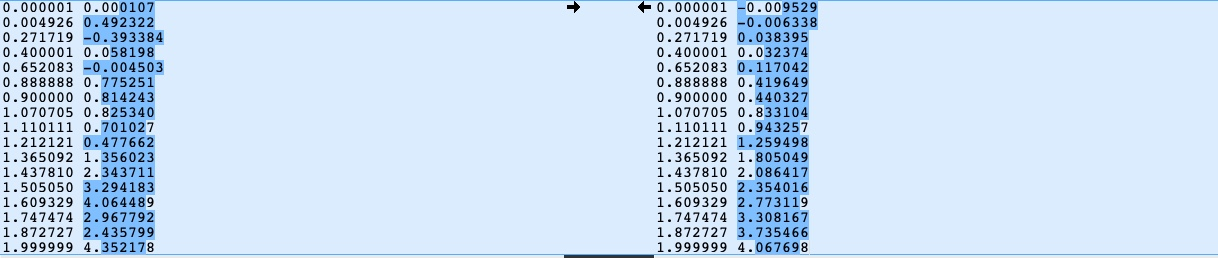
\includegraphics[width =\textwidth]{meld}
Сравнение предсказанных значений в произвольных точках отрезка на основе вычислений по разным методам c помощью \textit{meld}\\
Слева - интерполяция полиномом Лагранжа \\
Справа - аппроксимация методом наименьших квадратов \\

\indent \textbf{Функции}

\vspace{-\medskipamount}
\vspace{-2\baselineskip}
\vspace{10pt}
\usemintedstyle[c]{friendly} 
\begin{minted}{c}
long double
y_Lagrange(long double *x, long double *y, int num, long double x0) {
    long double L;
    int i, j;
    long double P;

    L = 0;
    for (i = 0; i < num; i++) {
        P = 1;
        for (j = 0; j < num; j++) {
            if (i != j) {
                P *= (x0 - x[j]) / (x[i] - x[j]);              
            }
        }
        L += y[i] * P;
    }
    return L;
}
\end{minted}
\\
\vspace{-\medskipamount}
\vspace{-2\baselineskip}
\vspace{10pt}
\usemintedstyle[c]{friendly} 
\begin{minted}{c}
long double
y_LeastSquares(long double *x, long double* y, int num, long double x0) {
    int i, j, k;

    for (i = 0; i < n + 1; i++){
        a[i]=0;
        b[i]=0;
            for ( j = 0; j < n + 1; j++){
                sum[i][j] = 0;
            }
    }

    for (i = 0; i < n + 1; i++) {
        for (j = 0; j < n + 1; j++) {
            sum[i][j] = 0;
            for (k = 0; k < num; k++) {
                sum[i][j] += pow(x[k], i + j);
            }
        }
    }
    
    for (i = 0; i < n + 1; i++) {
        for (k = 0; k < num; k++) {
            b[i] += pow(x[k], i) * y[k];
        }
    }

    long double temp = 0;
    for (i = 0; i < n + 1; i++) {
        if (sum[i][i] == 0) {
            for (j = 0; j < n + 1; j++) {
                if (j == i) {
                    continue;
                }
                if (sum[j][i] != 0 && sum[i][j] != 0) {
                    for (k = 0; k < n + 1; k++) {
                        temp = sum[j][k];
                        sum[j][k] = sum[i][k];
                        sum[i][k] = temp;
                    }
                    temp = b[j];
                    b[j] = b[i];
                    b[i] = temp;
                    break;
                }
            }
        }
    }

    for (k = 0; k < n + 1; k++) {
        for (i = k + 1; i < n + 1; i++) {
            if (sum[k][k] == 0) {
                printf("\n Solution doesn't exist! \n");
                return 0;
            }
            long double M = sum[i][k] / sum[k][k];
            for (j = k; j < n + 1; j++) {
                sum[i][j] -= M * sum[k][j];
        }
        b[i] -= M * b[k];
    }
}

    for (i = n; i >= 0; i--) {
        long double s = 0;
        for (j = i; j < n + 1; j++){
            s += sum[i][j] * a[j];
        }
        a[i] = (b[i] - s) / sum[i][i];
    }

    long double result = 0;

    for (i = 0; i < n + 1; i++){
        result += a[i] * pow(x0, i);
    }
    return result;
}

\end{minted}

\section*{Графическое представление результатов}


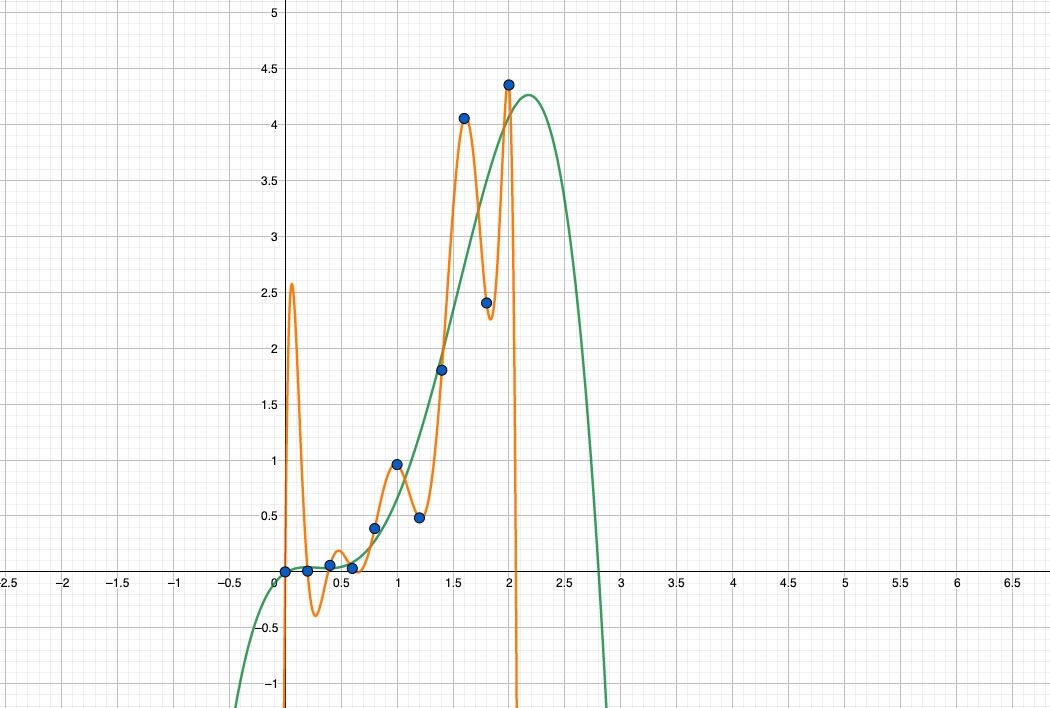
\includegraphics[width =\textwidth]{graphic}
Синие точки - точки, известные из условия \\
Оранжевая кривая - кривая интерполирующего многочлена в \\ форме Лагранжа \\
Зелёная кривая - кривая, построенная по методу наименьших квадратов

\section*{Анализ результатов}
\;\;\;\;\;\;Ключевым отличием двух рассматриваемых методов является то, что полином Лагранжа интерполирует функцию $f(x)$, точки которой нам известны, а метод наименьших квадратов эту функцию аппроксимирует. \\
\indentТо есть для полинома Лагранжа важно, чтобы полученная интерполяционная функция строго проходила через известные узлы, однако вне известных точек функция сильно "скачет". Такой разброс значений приводит к тому, что полученная интерполяционная кривая плохо характеризует поведение исходной функции $f(x)$ в целом. Это усложняет прогнозирование значений и дальнейшую работу с функцией, затрудняет визуальное восприятие графика.\\
\indentМетод наименьших квадратов, напротив, на выходе даёт нам такую функцию, которая лишь приближает $f(x)$, то есть может совпадать с рассматриваемой функцией на очень маленьком наборе точек, но зато полученная кривая довольно удобна и наглядна. 

\section*{Дополнительно: применимость методов}
\;\;\;\;\;\;В данный момент метод наименьших квадратов активно применяется в анализе данных. Этот метод помогает аппроксимировать различные экспериментальные данные в разных областях, например, в экономике. Это очень сильный инструмент, потому что позволяет сделать довольное точное прогнозирование новых значений. \\
\indentЧто касается интерполяции с помощью полинома Лагранжа, то такой метод тоже пользуется популярностью в современном мире. Например, метод был использован для вычислений при разработке двигателей. Построенный полином помог сократить количество реальных тестирований.

\section*{Источники и ресурсы}
Вводные лекции по численным методам (Д.П. Костомаров, A.П. Фаворский) \\
Для построения графика использовался ресурc \textit{www.geogebra.com}
\end{document}